\chapter{Practical Motivation}

Before jumping into the algorithm I would like to motivate the algorithm in an intuitive way.

I will introduce formal definitions of crease patterns and flat foldability in the next chapter.
For now let's very roughly say a creaes pattern is a sheet with creases that are assigned either mountain (M) or valley (V).
The creases (M/V) and borders of the paper (assignment = "B") are represented by edges of a planar graph.

As a very rough notion let's define that a crease pattern is considered to be flat foldable if there exists a configuration
of the paper such that each crease is folded according to its assignment and the paper does not intersect itself at any point.

We can represent a crease pattern by a planar geometric graph that has
\begin{itemize}
    \item{nodes at all the corners of the paper with straight edges between those. we will set their assignment to "B" (border).}
    \item nodes where any pair of creases intersect or where a crease touches the border of the paper.
    \item edges between nodes that represent parts or complete creases. When the "back of the crease" faces the observer we note down it's assignment as "M" (mountain crease). When if faces away it from the observer it's assigned "V" (valley crease).
\end{itemize}

(Note: add that this adds the constraint / assumes that all edges are straight; the borders of the crease pattern are straight)

\begin{figure}[h]
\centering
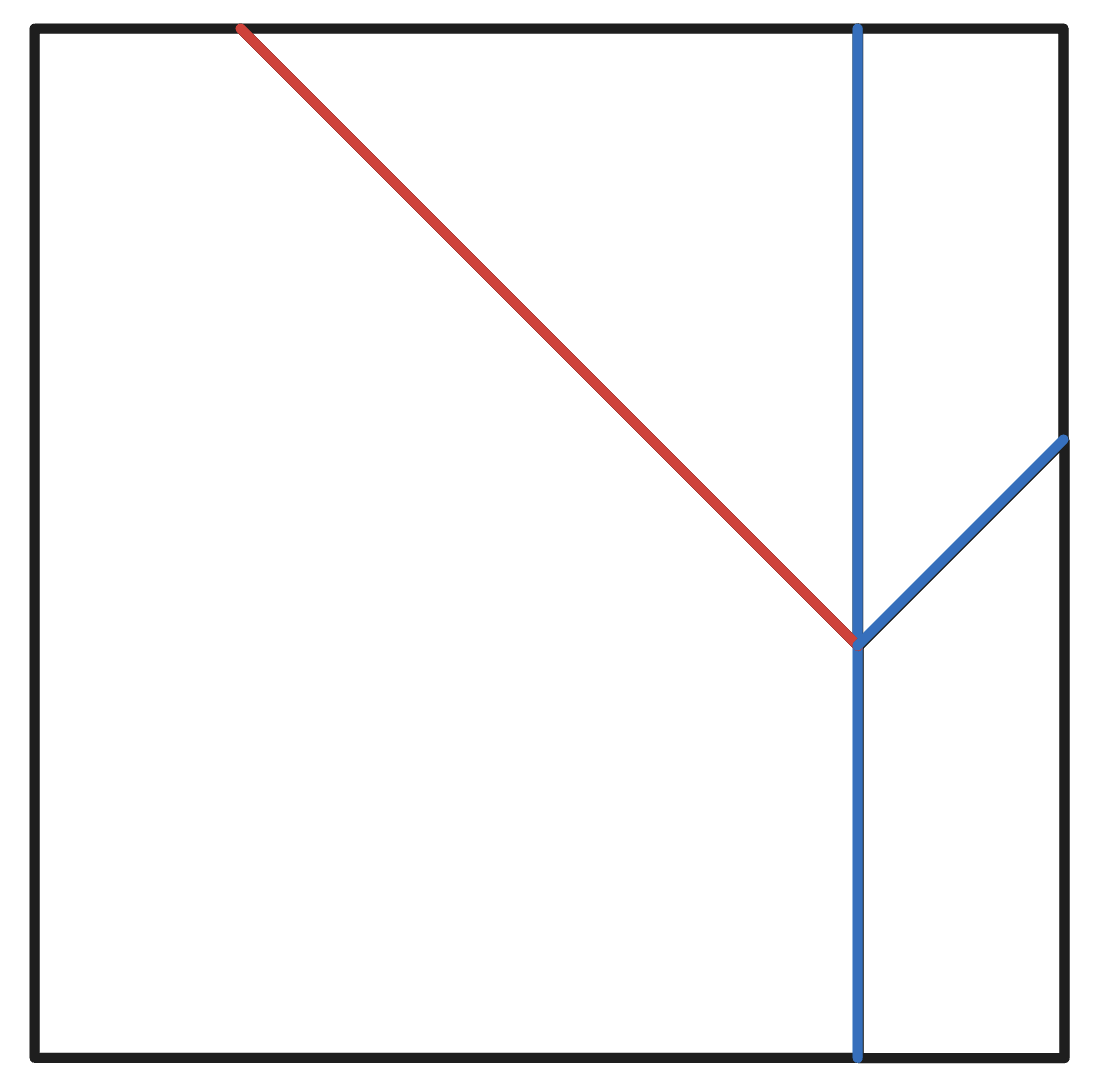
\includegraphics[width=0.4\textwidth]{assets/demo_creasepattern.png}
\caption{Example crease pattern that we want to determine the flat foldability of.}
\label{fig:demo_creasepattern}
\end{figure}

Let's say we get the crease pattern in Figure~\ref{fig:demo_creasepattern} and want to figure out - in a very hands on way - if this crease pattern is flat foldable.

To get a grasp of what a flatfolded configuration of the crease pattern might look like we can try to work out the general positioning of the faces relative to each other.

What I mean by that is that we use the face that a flat folded state will not introduce any new creases so we know every
uncreased area of the crease pattern will be a continious uncreased area in a flat folded configuration.

We also know about the creases that the paper here makes a 180 degree turn (ignoring any thickness of the paper) as any
other angle would elevate the folded structure into the 3rd dimension thus making it not a flat fold.

We can choose an arbitrary face as defining the frame of reference.
In this stage we're only interested in the relative position of the faces in the 2d plane in which the crease pattern is embedded.
To not get bogged down by the ordering of overlapping faces, let's free ourselves from the constraint that the paper is one continious / strongly connected object and only work with the shape of the faces for now.
Practically we might cut out each face. To not lose the crease information let's label the edges of each
face which connects to another face by what type of crease (M/V) it was and the id of the other face.

\begin{figure}[h]
\centering
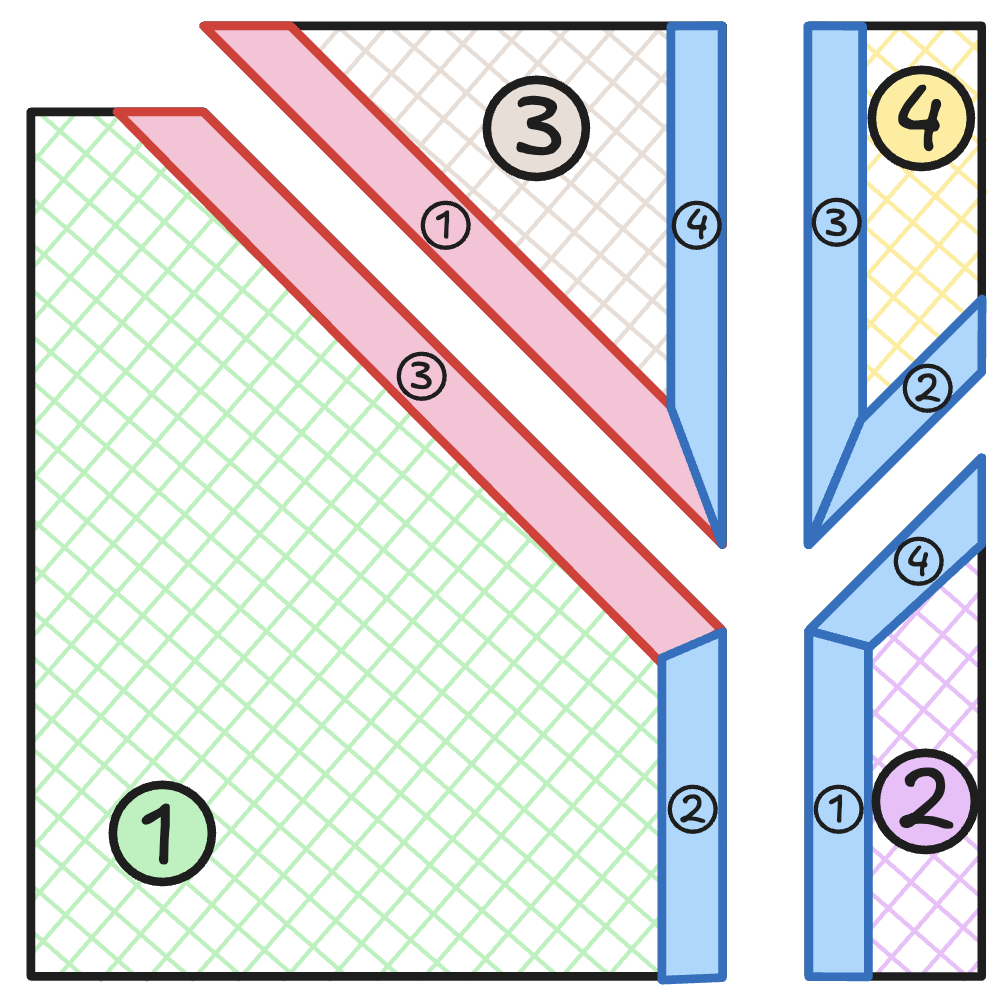
\includegraphics[width=0.4\textwidth]{assets/demo_faces.png}
\caption{Cut out faces of the crease pattern with face enumeration and edge labeling}
\label{fig:demo_faces}
\end{figure}

Continuing with the examplary crease pattern from Figure~\ref{fig:demo_creasepattern} this step looks like Figure~\ref{fig:demo_faces}.

We have seperated the different faces of the crease pattern and assigned them ids from 1 to 4.
Each edge that was part of a crease is colored according to the crease type (red = mountain; blue = valley) while noting down the originally neighbouring face.

Let's use face 1 as the frame of reference.
As face 1 borders face 2 at a valley crease we know that any flat folded configuration will feature face 2 mirrored along the edge overlapping face 1.

\begin{figure}[h]
\centering
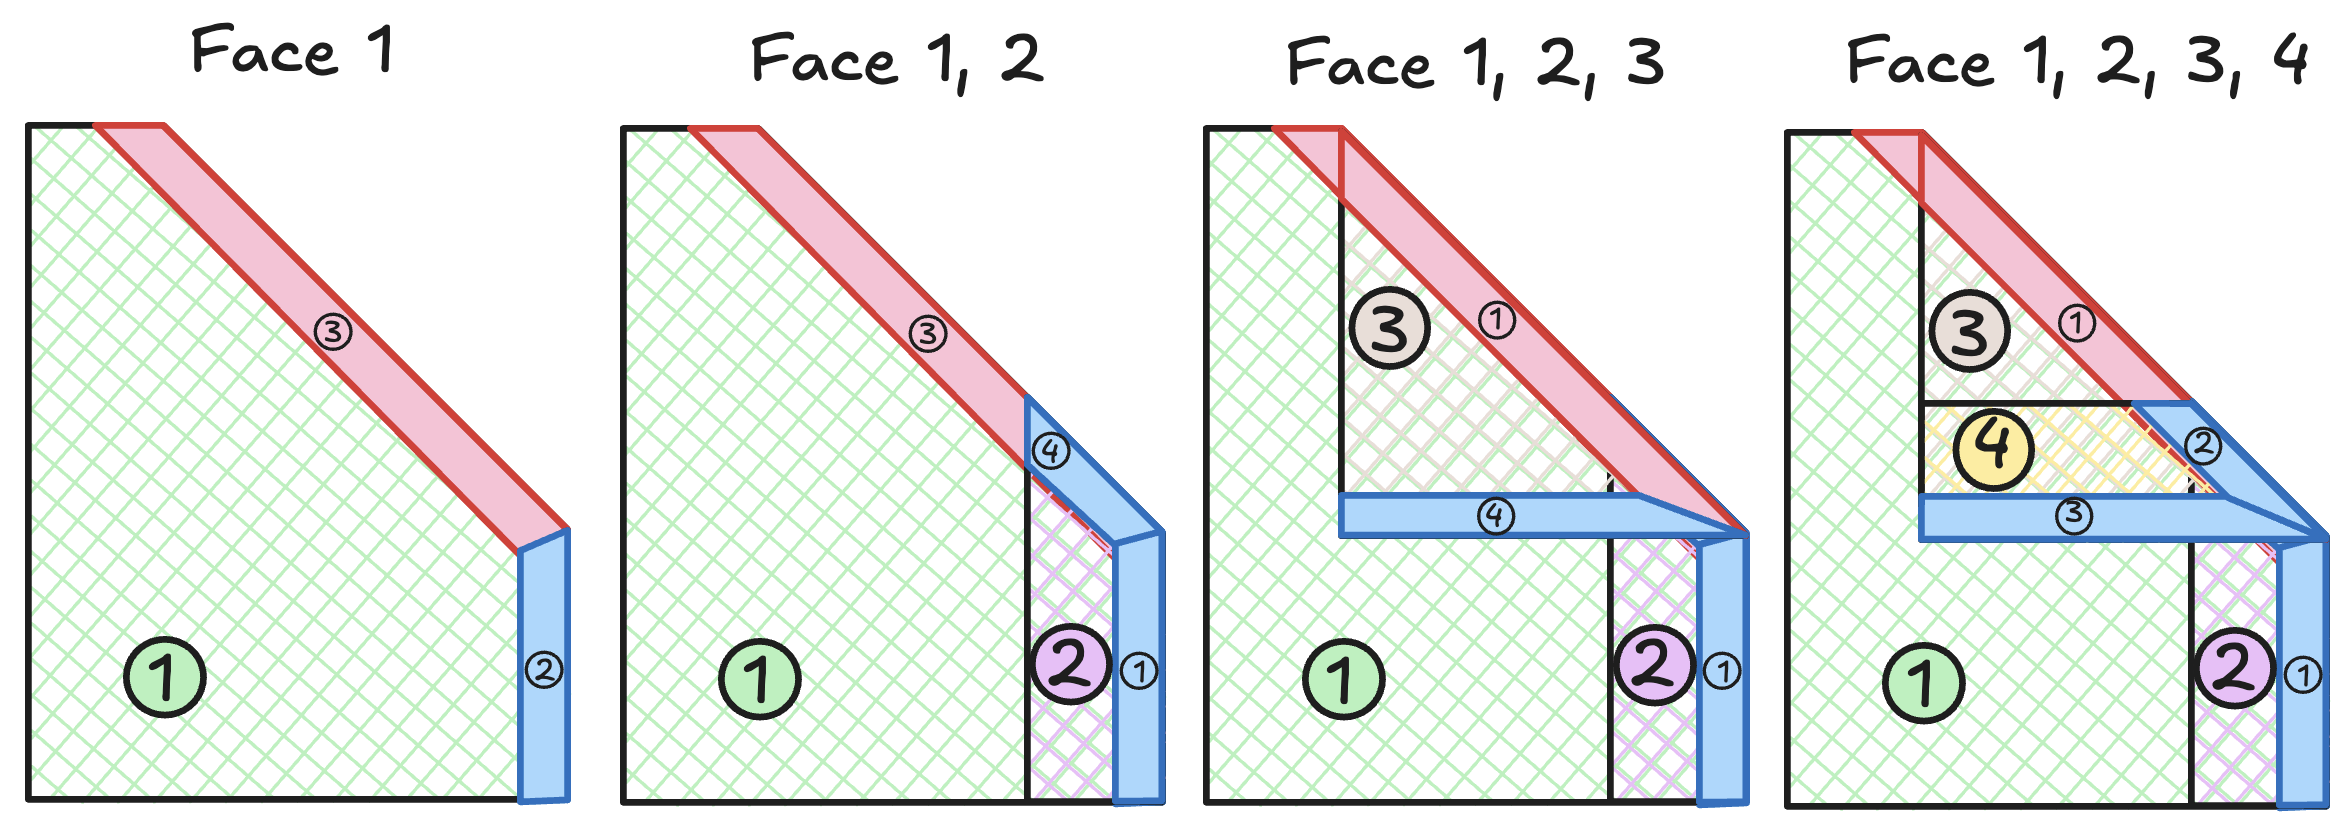
\includegraphics[width=\textwidth]{assets/demo_localflatfold.png}
\caption{Cut out faces of the crease pattern with face enumeration and edge labeling}
\label{fig:demo_localflatfold}
\end{figure}

By processing the faces in a neighbourly fashion (BFS / DFS / any other graph search on the face adjacency graph)
we know for certain where the next face will be located in the 2d plane.
This iterative construction is displayed step by step in Figure~\ref{fig:demo_localflatfold}.

In Figure~\ref{fig:demo_localflatfold} we can see this construction in 4 steps.

First we choose the face that defines the frame of reference and place it on the 2d plane.

Then we add face 2 which is neighbouring face 1. As they share the mountain valley to the right of face 1, the left edge
of face 2 aligns with this edge while the rest of face 2 extends to the left in order to fulfill the 180 degree that crease requires.

In the third step we position face 3 mirrored along the common edge with face 1.

Finally we position face 4 along the common edge with face 3.
As face 3 is already mirrored face 4 will be doubly mirrored aka not mirrored.

We could've used the common edge of face 4 with face 2 to find its relative positioning too.
In fact if a flat folded configuration exists at all then this will result in the same positioning.

This is a result of Kawasaki's theorem that states that the sum of alternating angles between the edges incident to a node must cancel out to zero. 
If by this process we position a face so that not all of its edges align with the corresponding edges of neighbouring faces
then we can already conclude that the crease pattern is not flat foldable.

Great! Now we have an intersection free configuration of the crease pattern, except we're dealing with cut out versions of the faces.
When reconnecting the faces we're not guranteed 

- davon ausgehend dass ich das physische modell mit der 3. dimension habe:
- mache klar, dass das ordering jetzt eher folge der construction steps ist
- garantiert keine intersection-freeness
- sollten alle orderings angucken

- dann können wir das contraint der edge types einführen
- zuletzt die taco / tortilla notion / betrachtugn / kategorisierung

So now it's about reconnecting the faces that share common edges.

For this first we need to introduce somewhat of a third dimension back into our model. The relative order of the faces is ignored / the physical mod

As we've already determined the relative positioning of the faces, finding a flat folding is now reduced
to finding a ordering of the original faces such that the paper does not intersect itself.

The only way the paper can intersect itself is in the crossection of a crease.

Let's cheat a little and look at the crossectional view of the flat folded configuration.

\begin{figure}[h]
\centering
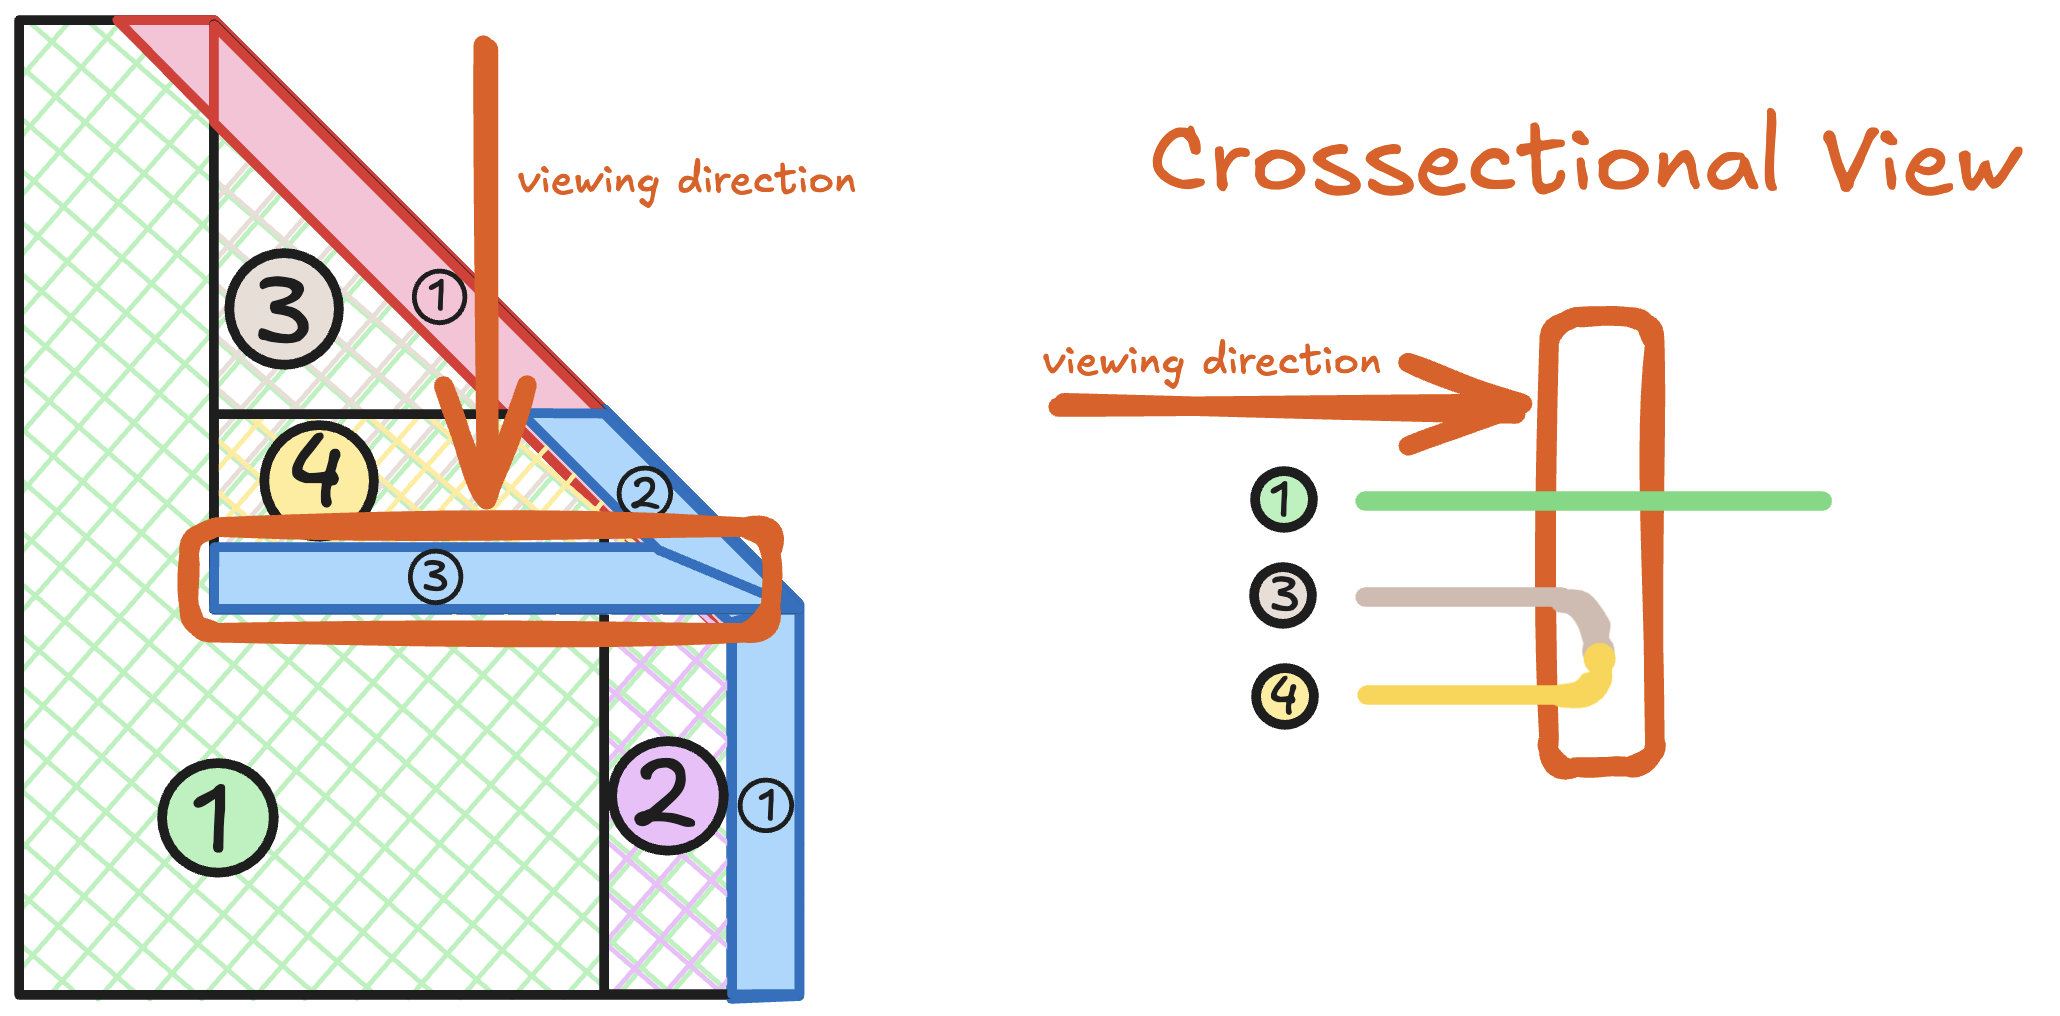
\includegraphics[width=0.6\textwidth]{assets/demo_csx_taco_tortilla.png}
\caption{Left: visual indication along which edge we look at the crossection of the system of faces; Right: Crossectional view along the highlighted edge; Face 1 is on top and penetrates the crossection, Face 4 is the bottom most face and forms a crease with Face 3 wich is layered in between Face 1 and 3.}
\label{fig:demo_csx_taco_tortilla}
\end{figure}

Looking at the crossection of the common edge of face 3 and 4 (see Figure~\ref{fig:demo_csx_taco_tortilla}) we see that face 1 penetrates the crossection while face 3 and 4 form a crease.
The crease between face 3 and 4 is a valley crease. Face 3 is mirrored while Face 4 is not.
Such we can confirm that this is a valid ordering of the faces (intersection free) and btw that any valid ordering must put face 3 above face 4.

\begin{figure}[h]
\centering
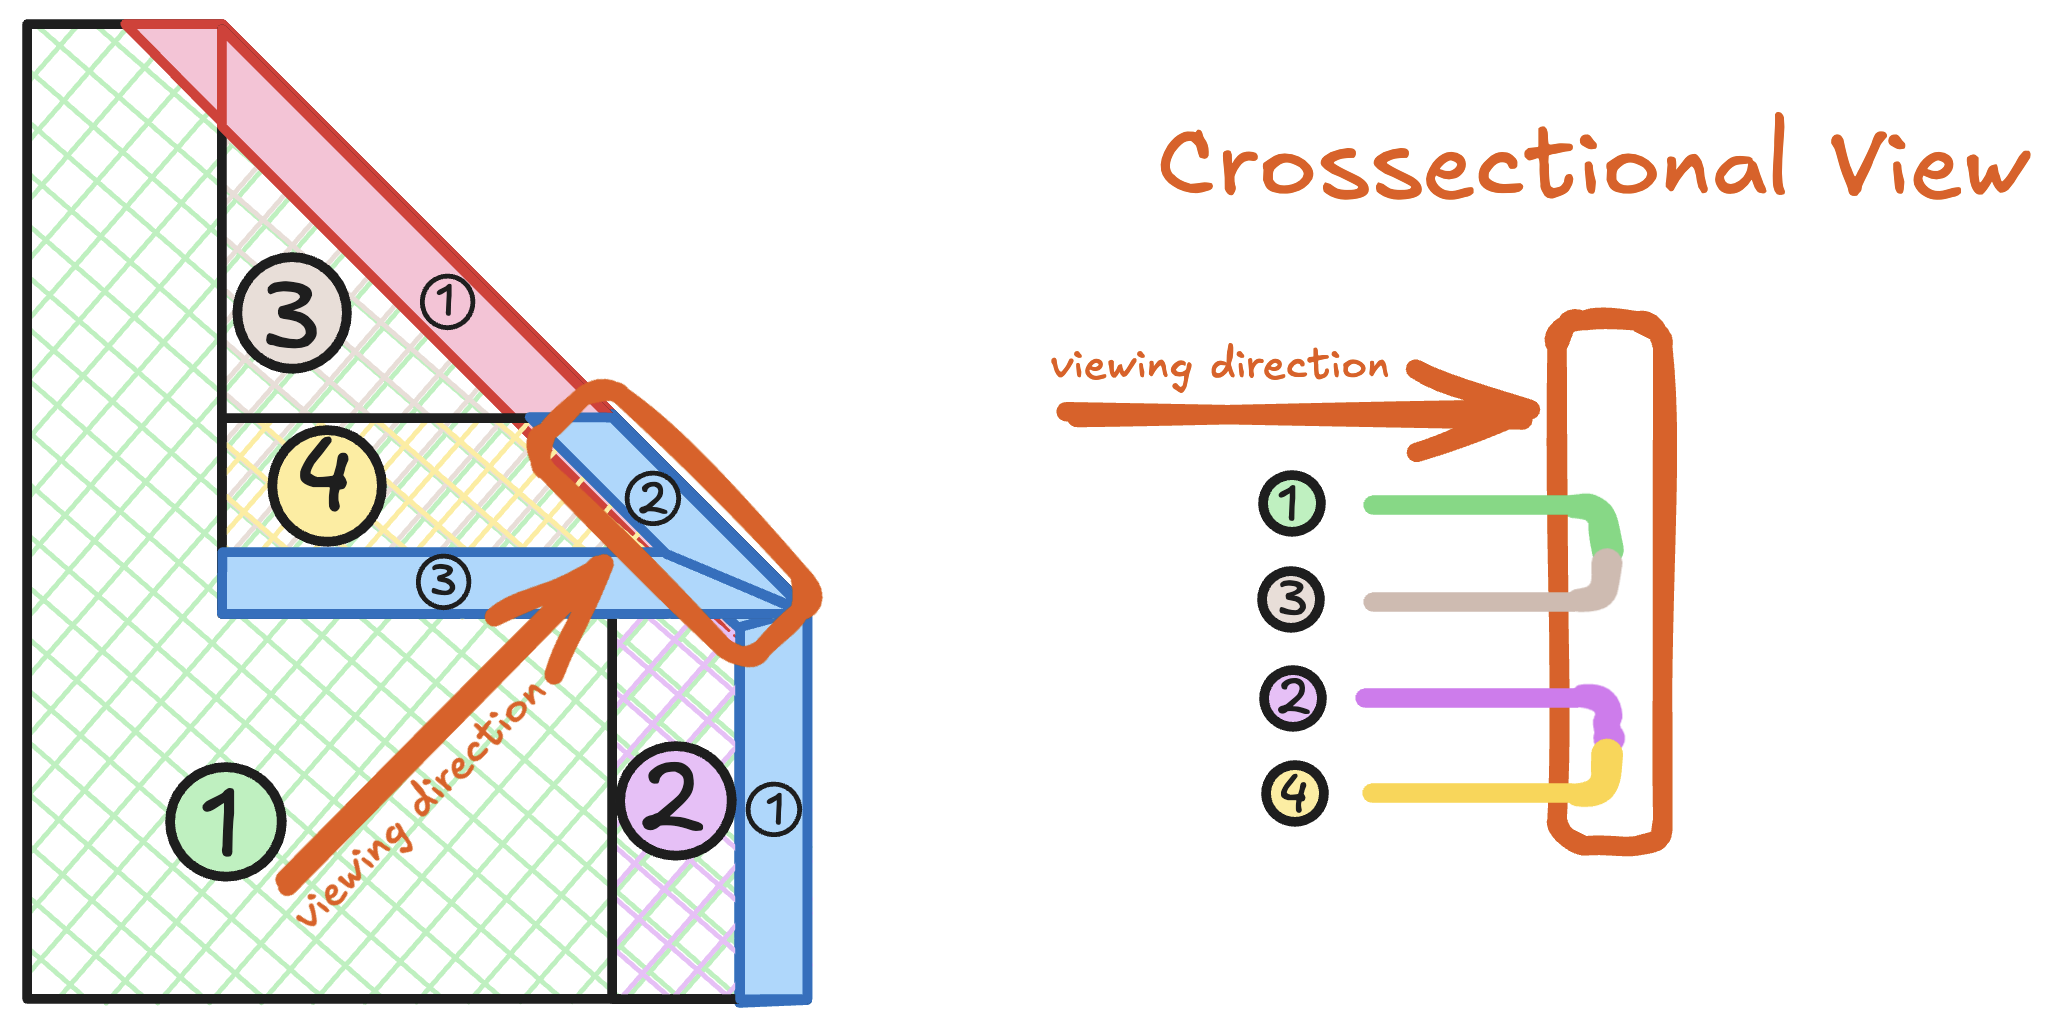
\includegraphics[width=0.6\textwidth]{assets/demo_csx_taco_taco.png}
\caption{Left: visual indication along which edge we look at the crossection of the system of faces; Right: Crossectional view along the highlighted edge; Face 1 and 3 are on top and connect to form a crease. Face 2 and 4 are below both and also connect to form a crease.}
\label{fig:demo_csx_taco_taco}
\end{figure}

Looking at the crossection of where both the crease between face 2 and 4 and part of the crease between the faces 1 and 3
land we can in the same way confirm that the crease assignment is obeyed as face 1 is above face 3 and face 2 is above face 4.

While making sure that the crease assignment is obeyed at all crossections is great we can use it to confirm the ordering is intersection free.

The two possible violations that can occur here can be categorized into 2 kinds.
As shown in the left in Figure~\ref{fig:demo_csx_bad_ordering} one kind of violation would be a face that penetrates a crease.
Here face 1 is between face 3 and face 4 but face 3 and 4 must form a crease in this crossection.

On the right side of Figure~\ref{fig:demo_csx_bad_ordering} you can see the other kind: two pairs of faces that form a crease in this cross section are interleaved.
This creates a self intersection of the paper.
 
\begin{figure}[h]
\centering
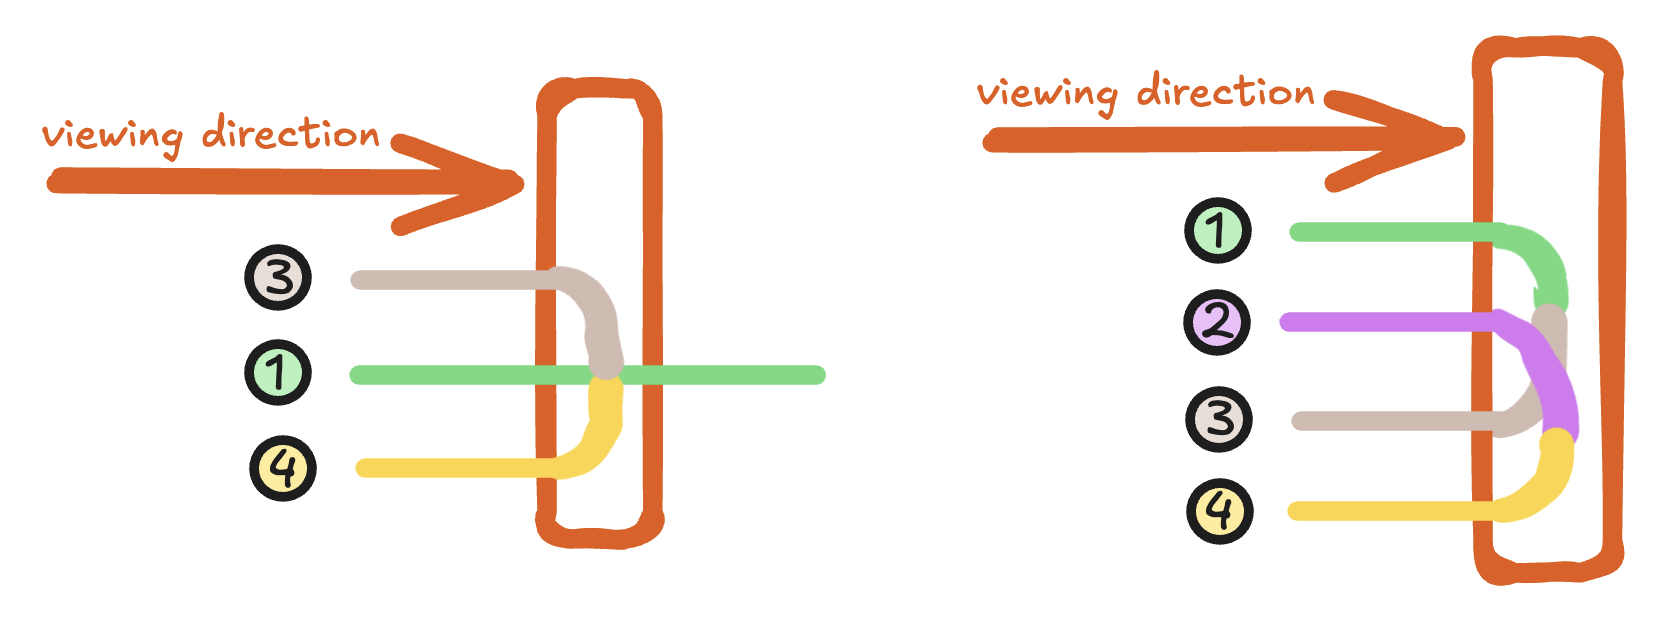
\includegraphics[width=0.6\textwidth]{assets/demo_csx_bad_ordering.png}
\caption{Alternate face orderings that create self intersections in the crossection examined in Figure~\ref{fig:demo_csx_taco_tortilla} (left) and in Figure~\ref{fig:demo_csx_taco_taco} (right).}.
\label{fig:demo_csx_bad_ordering}
\end{figure}
